\begin{figure}[t]
   \centering
   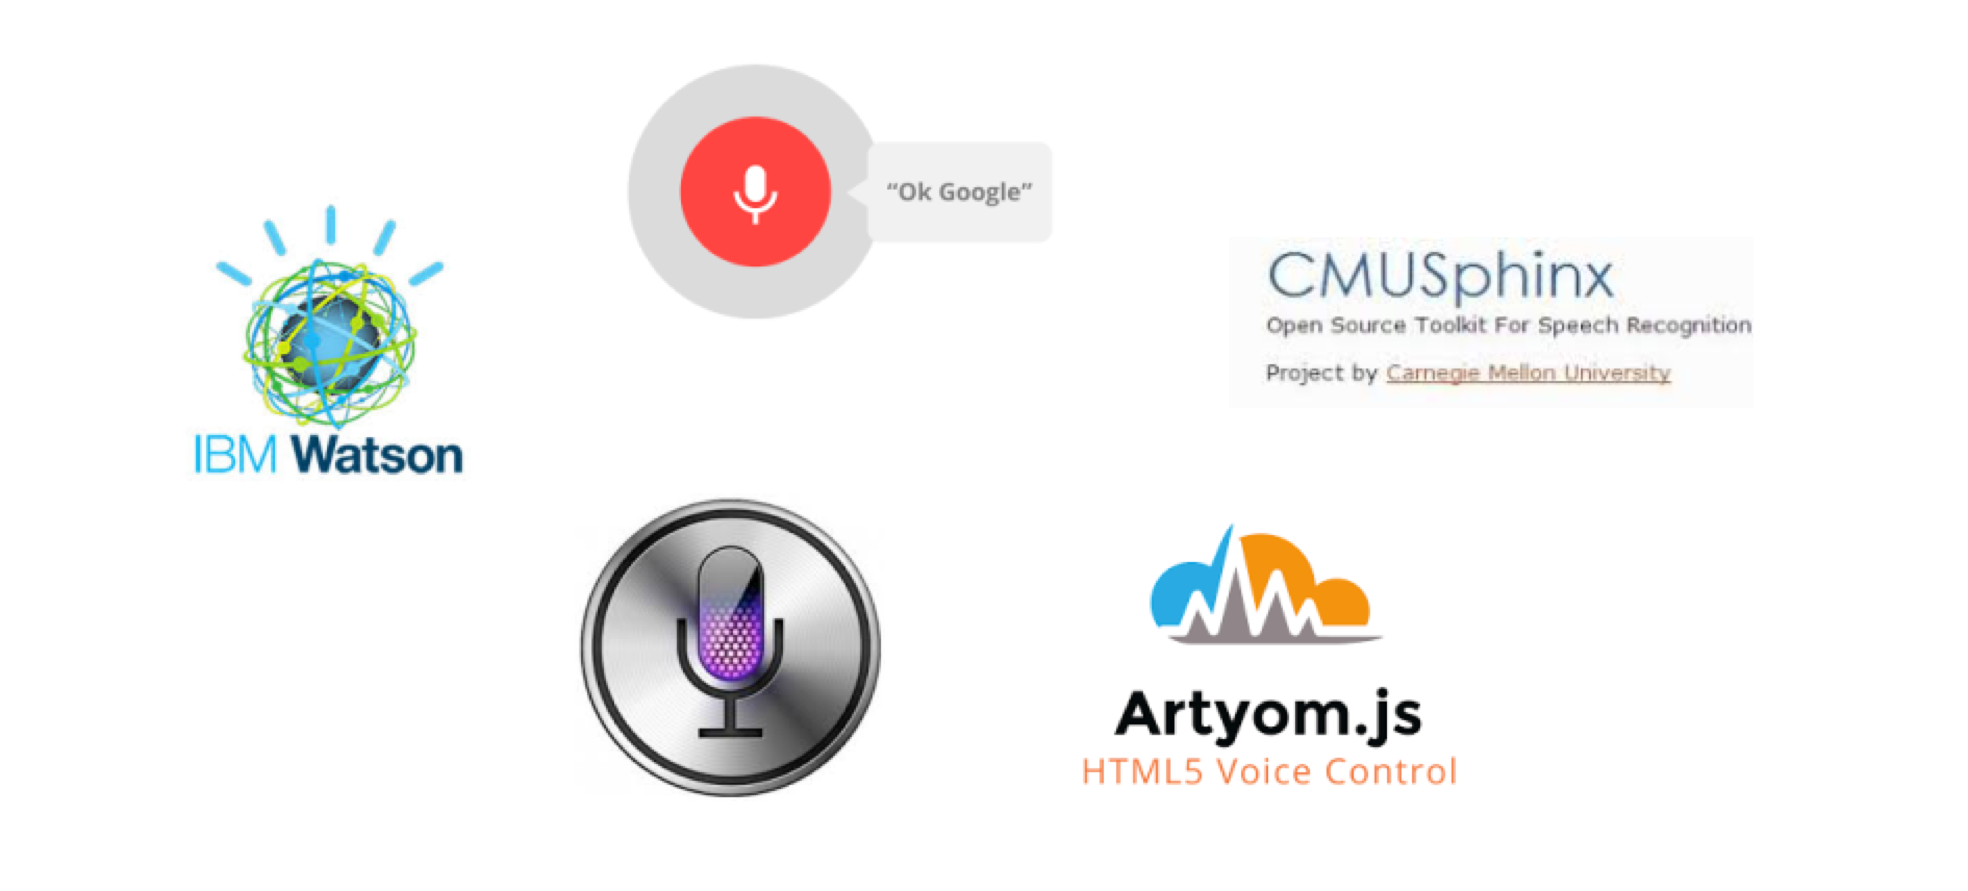
\includegraphics[width=\columnwidth]{figures/Picture2.png}.
   \caption{A few speech recognition services.}
   \label{fig:speechrecognizers}
\end{figure}

\section{Previous Work}
\label{sec:previous}

Previous work in breaking audio CAPTCHAs involved the use of \textit{Hidden Markov Models (HMMs)} or \textit{Artificial Neural Networks} (ANNs) to perform automatic speech recognition on segments of the CAPTCHA. To apply these classification methods, initially the input signal is first segmented into a series of overlapping frames to extract feature vectors. The three feature representations that are currently relied upon are Mel-Frequency Cepstral Coefficiants (MFCC), Perceptual  Linear  Prediction  (PLP),  and relative  spectral  transform-PLP  (RAS TA-PLP). Using HMM-based ASR[6], Hendrik et al achieved an accuracy of 62.8\% with Google's reCAPTCHA (2014 version). A later paper by Hendrik et al also exploited semi-supervised learning techniques as a cost-effective alternative to break audio CAPTCHAs[7]. \newline

Tam et al[1, 2] created their own classification system, training their data set on scraped CAPTCHAs.[1] Bursztien et al[8] adopted a two-stage approach to solving audio CAPTCHAs, first segmenting the audio file into parts and then getting the individual transcriptions for each of the parts using a classification algorithm. They evaluated their system which they called DeCaptcha, against six audio CAPTCHA systems and broke five of them, all with more than 40\% accuracy.\newline

Other previous work, relied on modifying existing off the shelf tools such as the CMU sphinx speech recognizer[5], using machine learning to improve its accuracy to 75\%. It was observed that CMU Sphinx without the help of machine learning was able to give an efficiency of 9.6\% with the TIDIGITS model, and 28.9\% with the HUB4 model. \newline

Thus, all these systems found performance of off-the-shelf tools unreliable and inefficient and relied on machine learning techniques to build their solvers. Our approach exploits features in existing speech recognition services to solve audio CAPTCHAs with a higher level of accuracy than all previous studies. We are looking at noise reduction and deep learning as avenues of improvements over our obtained results.




